
%% technical_analysis_of_ghanapost_gps.tex
%% V1.0
%% 2017/10/28
%% by Archzilon Eshun-Davies(laudarch)

%%*************************************************************************
%% Legal Notice:
%% This code is offered as-is without any warranty either expressed or
%% implied; without even the implied warranty of MERCHANTABILITY or
%% FITNESS FOR A PARTICULAR PURPOSE! 
%% User assumes all risk.
%%*************************************************************************


\documentclass[conference,compsoc]{IEEEtran}


\ifCLASSOPTIONcompsoc
  % IEEE Computer Society needs nocompress option
  \usepackage[nocompress]{cite}
\else
  % normal IEEE
  \usepackage{cite}
\fi

\ifCLASSINFOpdf
   \usepackage[pdftex]{graphicx}
  \graphicspath{{./figures/}}
  \DeclareGraphicsExtensions{.pdf,.jpeg,.png}
\fi

\usepackage{url}


\hyphenation{op-tical net-works semi-conduc-tor on-line}


\begin{document}

\title{Technical Analysis of\\ GhanaPost GPS (AsaaseGPS)}

\author{\IEEEauthorblockN{Archzilon Eshun-Davies (laudarch)}
\IEEEauthorblockA{Qremia Evolution\\
Accra, Ghana\\
Email: \url|laudarch@qremiaevolution.org| \\
Website: \url{http://qremiaevolution.org}}}

% make the title area
\maketitle

% As a general rule, do not put math, special symbols or citations
% in the abstract
\begin{abstract}
This paper seeks to investigate and analyze the technical details of the GhanaPost GPS application and try to give recommendations on how the system could be made better, 
this paper also demonstrates that the technologies used to build the solution
has drastic implications whereas if careful attention was given, a stronger and more secure solution could have been achieved. I also try to debunk the current argument of progressive development.
\end{abstract}

% no keywords
\begin{IEEEkeywords} 
	AsaaseGPS, Ghana Post, Digital address. 
\end{IEEEkeywords}


\section{Introduction}
\IEEEPARstart
"GhanaPostGPS is Ghana’s official digital property addressing system which covers every inch of the country and ensures that all locations in the country are addressed. With GhanaPostGPS, every location has a unique digital address."\cite{ghanapost:about}
\newline

This is certainly a very modest idea but in this paper we would look at security and architecture of the system; while at the same time hinting on Data security for the Ghanaian.
\newline
This paper in no way dismisses the work done by the developers of "GhanaPostGPS".

\section{Architecture}
Before any system is built it must be designed first. The idea of what goes where
needs to be visually drawn in order to not sway from it or end up with a broken
system. Any architecture must have 3 fundamental properties\newline
* It must have a core\newline
* Abstraction for the core\newline
* and Finally the initial plan\newline
\newline
If the core architecture is not defined well, changes to the core would be made in the short and long term which
renders the core design useless.

The GhanaPostGPS architecture as seen in (Figure.\ref{fig:arch_overview})
\newline 
\begin{figure}[h!]
	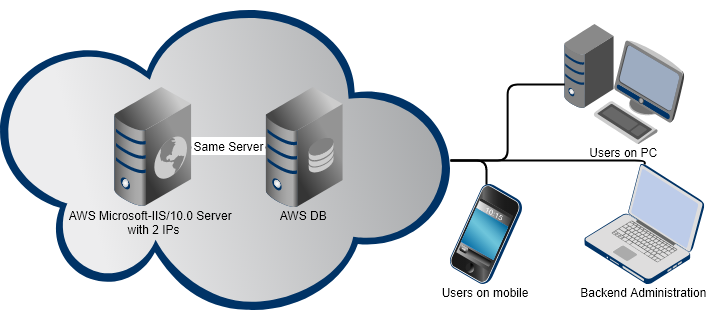
\includegraphics[width=2.5in]{architecture_overview}
	\caption{Architecture Overview.}
	\label{fig:arch_overview}
\end{figure}
\newpage
Developers of the system seem to have taken the easiest path and designed the
system as they would a traditional web application without consideration for
scaling and High Availability(HA).\newline With the aim of the project becoming a national requirement the developers should have factored that into their design.
\newline
It should be said though, that the Developers did make an attempt at load balancing using the DNS method as seen in (table.\ref{dns_lbd})

\subsection{Tools Used(ServerSide)}
On the Server Side the developers chose a .Net(dotnet) framework running on Microsoft's IIS Server; as can be seen in (table.\ref{table_serverside}). Even though
these are common platforms used in many deployments its usage globally has been declining in the past few years in favour of more robust and stable platforms. 
In recent times Windows has discontinued either its platforms or development tools\cite{dotnet45:ended} \cite{dotnet45:ended2} \cite{windowsphone:discontinued} \cite{kinect:ended}, and in some cases both. It is therefore careless to not consider all these facts when deciding on what systems to base a National service on. A more modern development tool(s) would have allowed for guaranteed time support and usage. \newline

The developers also used MySQL or MSSQL (as I have not verified this yet); if they did use any of these database engines, then it should be noted that, even though facebook and twitter initially run with these platforms they have long learnt from their mistakes and are using more bespoke and modern solutions like NoSQL.
\newline
The System seems to also be running on a single instance of AWS(Amazon Web Services). \newline I'll talk about the security implications later.


\subsection{Tools used (Client Side)}
I only investigated Android. The android client is written in B4A 
\footnote{B4A (Basic 4 Android) was written by "AnyWhere Software" as a wrapper for android for developers who are used to programming in Basic and can't or don't want to change to Java}\cite{b4awebsite}, it should be noted that the developer has experience in B4A. I believe B4A was used for portability but there are better options which are best suited for this type of application. Google Maps is re-used in the android client\footnote{It uses Google Maps API V2 with the API key AIzaSyAn\_vsgpw36hMASIgNgjUk8vdw4ljhJGxA}. \newline

The Android client is designed to open the urls specified in (table.\ref{table_androidurls})
\newline

\begin{table}
	\renewcommand{\arraystretch}{1.5}
	\caption{Client side URL Handlers}
	\label{table_androidurls}
	\centering
	\begin{tabular}{|c|c|}
		\hline 
		URI & SCHEME \\
		\hline
		asaasegps.com & asaasegps \\ \hline
		www.asaasegps.com & https \\ \hline
		www.gps.ghanapost.com.gh & https \\ \hline
		gps.ghanapost.com.gh & ghanapostgps \\ \hline
		www.ghanapostgps.com & https \\ \hline
		ghanapostgps.com & ghanapostgps \\ \hline
		www.ghanapostgps.com.gh & https \\ \hline
		ghanapostgps.com.gh & ghanapostgps \\ 
		\hline
	\end{tabular}
\end{table}

For some reason they designed custom schemes "asaasegps://", "ghanapostgps://" et al as specified in (table.\ref{table_androidurls})

The Client also opens the website even though it has near native code that is suppose to handle that.

\section{Security}
I will consider security in terms of System and user.The "System" would be in reference to server side and client side whereas "user" would be about anything that is user centric.
The system lacks a lot of security checks; so much so that I believe security was not part of the fundamental design consideration.\newline

The location is based on Google's OpenLocation\cite{openlocation:website} \cite{openlocation:website2} Code\footnote{
Open Location Codes are short, 10-11 character codes that can be used instead
of street addresses. The codes can be generated and decoded offline, and use
a reduced character set that minimizes the chance of codes including words.

Codes are able to be shortened relative to a nearby location. This means that
in many cases, only four to seven characters of the code are needed.
To recover the original code, the same location is not required, as long as
a nearby location is provided.

Codes represent rectangular areas rather than points, and the longer the
code, the smaller the area. A 10 character code represents a 13.5x13.5
meter area (at the equator. An 11 character code represents approximately
a 2.8x3.5 meter area.

Two encoding algorithms are used. The first 10 characters are pairs of
characters, one for latitude and one for longitude, using base 20. Each pair
reduces the area of the code by a factor of 400. Only even code lengths are
sensible, since an odd-numbered length would have sides in a ratio of 20:1.

At position 11, the algorithm changes so that each character selects one
position from a 4x5 grid. This allows single-character refinements.
} with slight definitions specific to Ghana; Using and open system like this means one does not even need the application to generate ones own addresses.

On the server side the admin is exposed on  \url|https://www.ghanapostgps.com/admin| as seen in (figure.\ref{fig:admin_login}) \newline
there is no capture apart from a CRSF\footnote{Cross Site Scripting Forgery} token, which does not really protect from a "brute force" attack.
%\pagebreak
\begin{figure}
	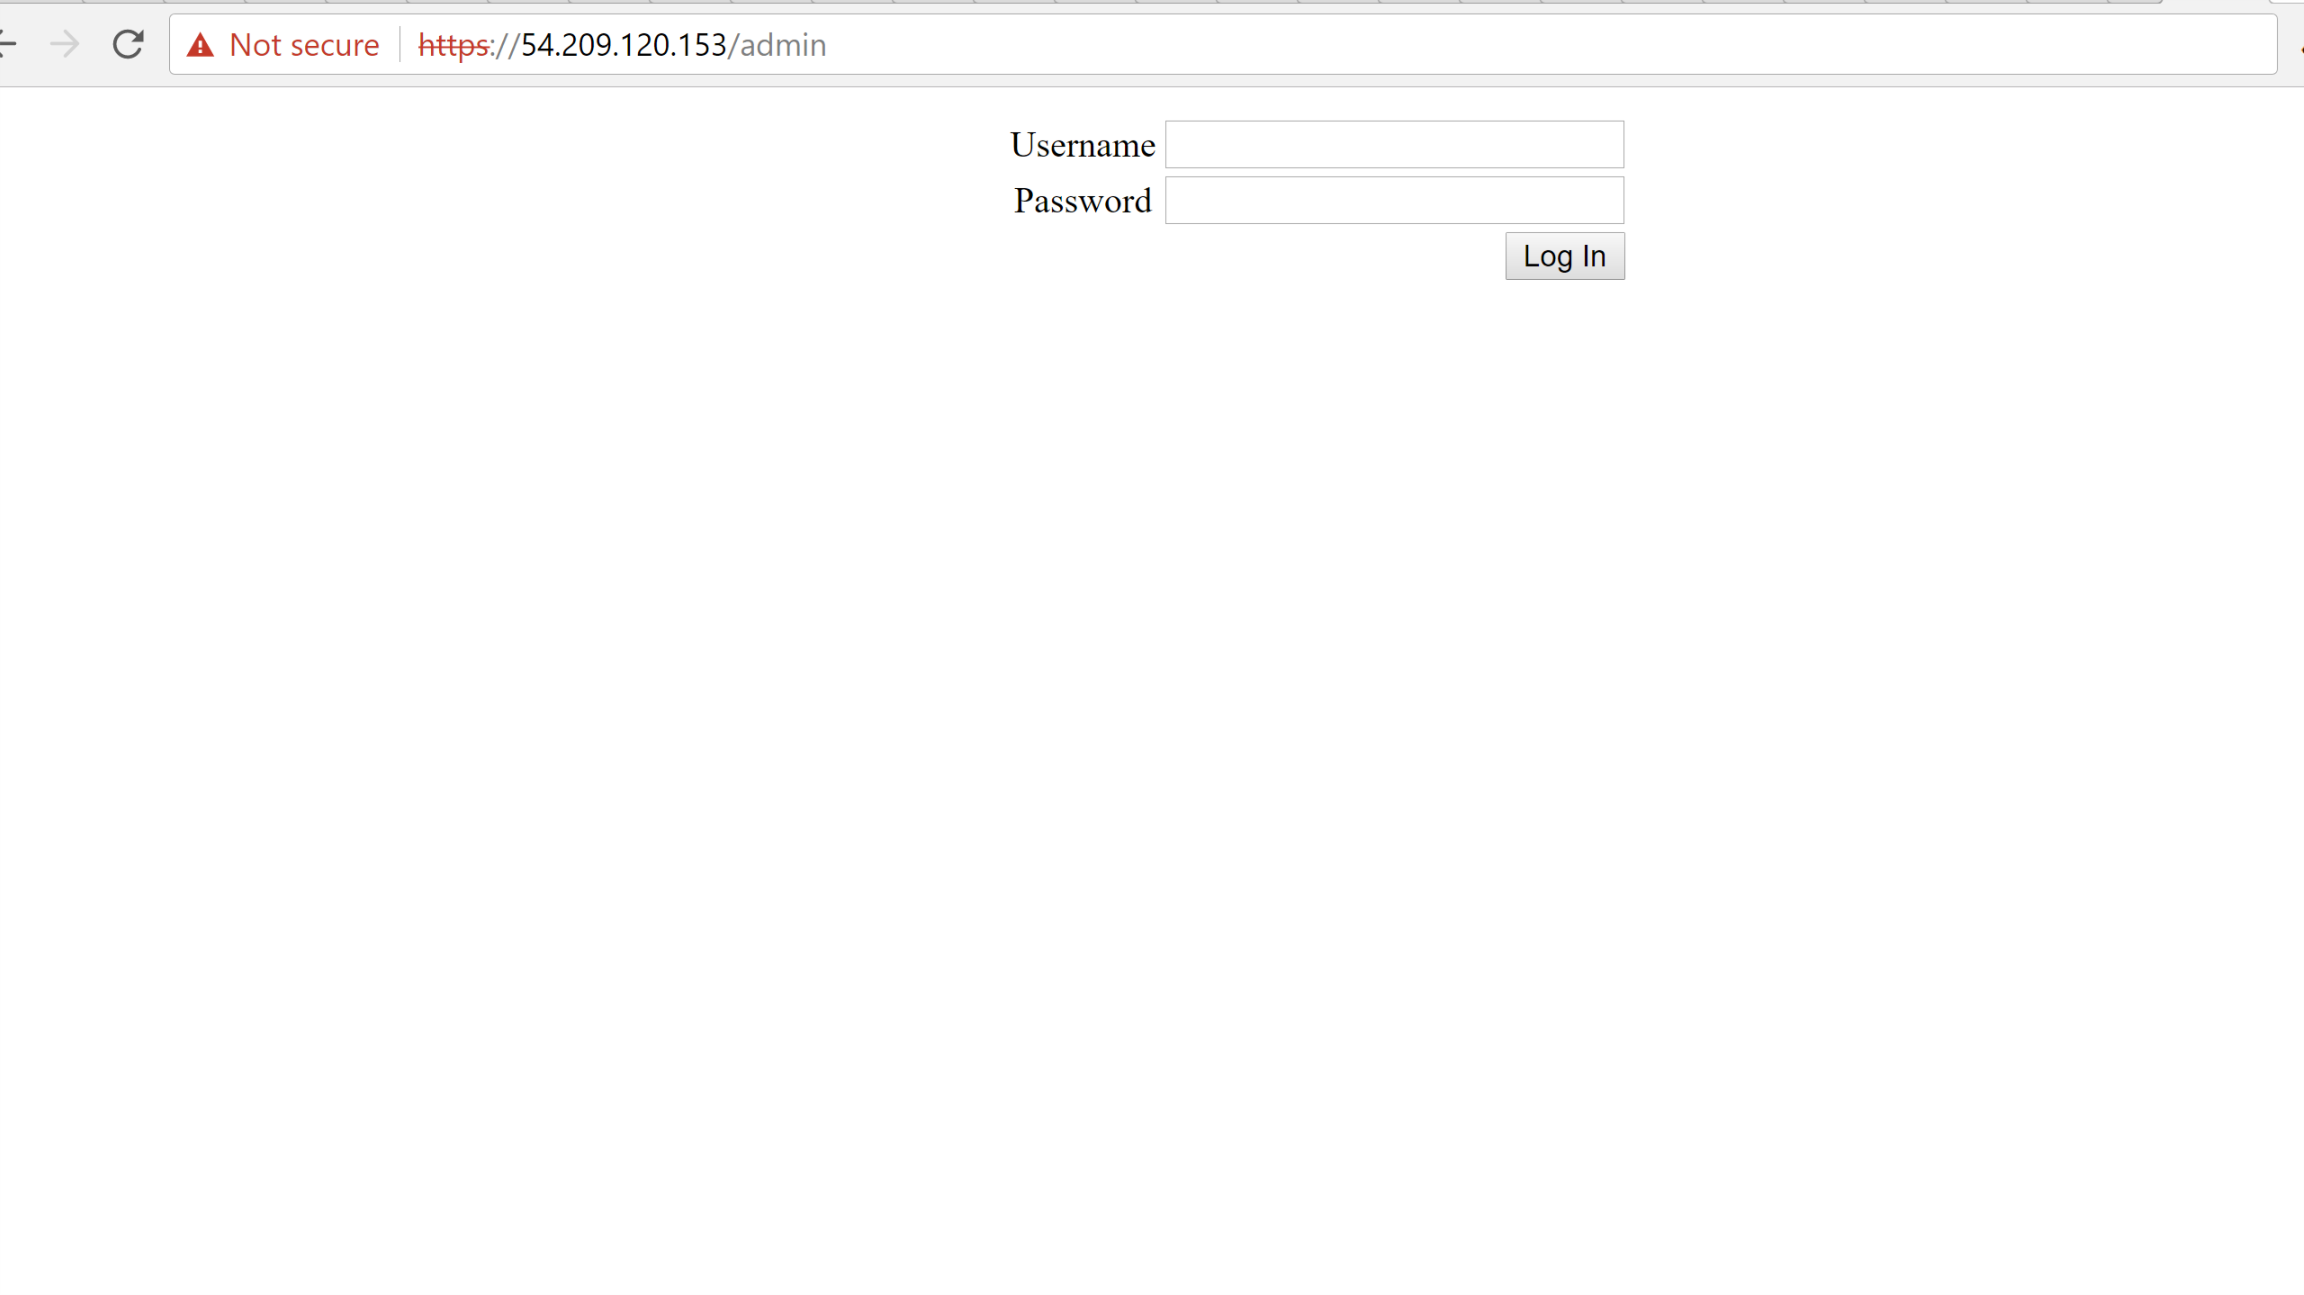
\includegraphics[width=3.5in]{admin_login}
	\caption{Admin login.}
	\label{fig:admin_login}
\end{figure}

The services are hosted on foreign territory therefore Ghanaian data would not be Governed by the Data Protection Laws\cite{dataprotection:ghana} of Ghana. The European Data Protection Laws\cite{dataprotection:europe} takes precedence and do not match the Ghana Data protection Laws\cite{dataprotection:ghana}. The data stored on these servers are kept for a maximum of 5 years under the European laws and can be held further without notification to the developer or the Ghanaian.

This problem also affects the usage of Google Maps; we are in a monitored world and the western world is more autocratic in on-line services than any other, Google retains the data provided willingly and uses these data for targeted marketing and other known and unknown purposes, this means that; by just opening the app google already has your data and on top of that we are providing our GPS locations freely. This is clearly stated in the Google Maps privacy rules.
\newline
User tagging\footnote{User tagging has seen a boost in recent times and is used by almost all the top on-line services to track user movements without user notification or authorization} technology makes it easy for anyone to be able to track any user on-line and with the help of GhanaPostGPS to their very doorstep.
 
I believe careful analysis should have been done for a National project with sensitive Citizen data and it should have had a higher priority than the "Version 1" concept.

\subsection{Data}
As stated above the data stored no longer belongs to the Ghanaian but to foreign governments and entities regardless of whether they are allies or not.
This data is also not very well protected and therefore stands a good chance of being accessed by crackers; this means we the Ghanaian are going to have our identities stolen and sold on the black market.

\subsection{Possible Attacks}
Potential attacks include but are not limited to DDoS attacks, Direct Attacks,
Data theft, impersonation.

\begin{table}[!t]
	\renewcommand{\arraystretch}{1.3}
	\caption{DNS Load Balancing Strategy}
	\label{dns_lbd}
	\centering
	\begin{tabular}{|c|c|}
		\hline
		ghanapostgps.com & 54.209.120.153\\
		\hline
		ghanapostgps.com & 54.88.252.118\\
		\hline
	\end{tabular}
\end{table}

\begin{table}[!t]
	\renewcommand{\arraystretch}{1.3}
	\caption{Server Side tools}
	\label{table_serverside}
	\centering
	\begin{tabular}{|c|c|}
		\hline
		Server & Microsoft-IIS/10.0\\
		\hline
		Database & MSSQL/MYSQL\\
		\hline
		Language & .NET/ASP.NET \\
		\hline
	\end{tabular}
\end{table}

\begin{table}[!t]
	\renewcommand{\arraystretch}{1.3}
	\caption{Client side tools}
	\label{table_clientside}
	\centering
	\begin{tabular}{|c|c|}
		\hline
		Platform & Android/IPhone\\
		\hline
		Map Engine & Google Maps\\
		\hline
		Language & B4A \\
		\hline
	\end{tabular}
\end{table}


\section{Conclusion}
So in conclusion, I choose not to be too detailed but at least demonstrate the dangers and bad design tactics that were used to build the system. I hereby propose the desired architecture and system design that can mitigate all these issues and more. \newline

NITA\footnote{National Information Technology Agency} \cite{nita:aboutus} has a Datacenter that has been designed to handle systems of this scale, and systems that hold National Data.

The proposed system would take into consideration security. In the design we assume here that physical security is taken care of and properly catered for by NITA.

Before we continue lets look at the issue of progressive development. It is believed among a certain group of the developer community
that projects should start with barely any functionality and progress as time goes on, this idea is normally referred to as the "Version 1" concept also known as the waterfall cycle except the part about specification and design is ignored to try and impress with rapid UI\footnote{User Interface} development. But as time has proven over and over again these ideas never work because
they do not consider the fundamentals of architecture design and are never implemented well.
\newline

\begin{figure}
	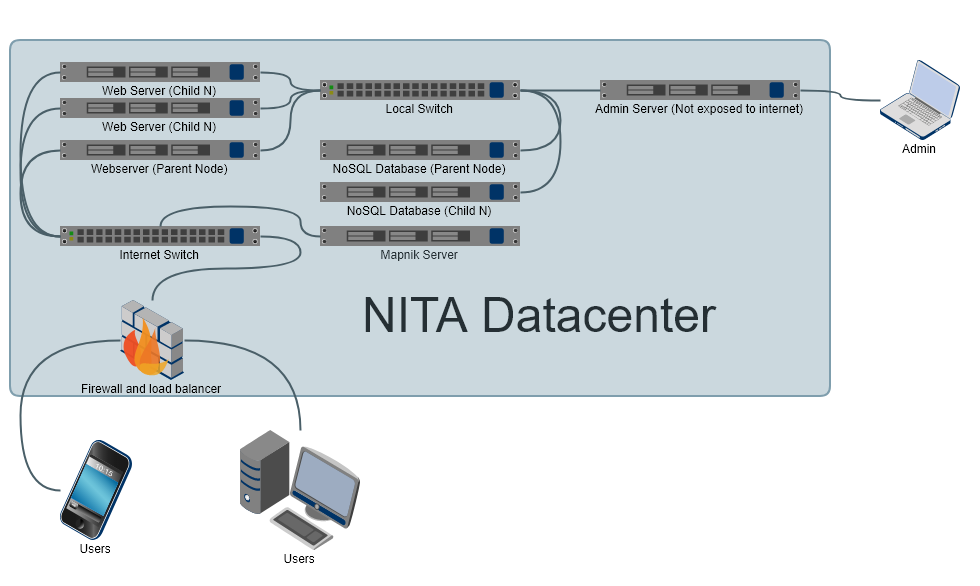
\includegraphics[width=3.5in]{proposed_arch_overview}
	\caption{Proposed Architecture Overview.}
	\label{fig:arch_proposed}
\end{figure}


Figure \ref{fig:arch_proposed} shows the proposed architecture while table \ref{proposed:arch} shows the proposed technologies to use. The proposed system uses a distributed architecture.
It proposed to have the admin side of the system only exposed to the internal network. The database is also to be
exposed only to the internal network. The reason why we only expose these services to the internal net work is
because they pose a serious security risk when exposed to the Internet, and there is no need for them to be
exposed to the Internet since its hosted locally at NITA.
\newline

The system also takes advantage of the distributed property of NodeJS applications where replicas of the same
application can be used as a superior form of High Availability and Scaling.
\newline

The admin node is also a separate server in order to avoid excessive administration work coinciding with user
activity. This design also allows for proper checks and accountability should there be an incident.
\newline

For the Map engine, I "highly" recommend using Mapnik\cite{mapnik:site}. Mapnik allows us to host our own map
engine and service which is similar to Google Maps and is used by OpenStreet Map\cite{openstreetmap:site}.
\newline


\begin{table}
	\renewcommand{\arraystretch}{1.5}
	\caption{Proposed Tools and setup Serverside \& Clientside}
	\label{proposed:arch}
	\centering
	\begin{tabular}{|c|c|}
		\hline
		Server & NodeJS\\
		\hline
		Map engine & Mapnik \\
		\hline
		Database & MongoDB/CouchDB\\
		\hline
		Language & Javascript \\
		\hline
		Load Balancer & Firewall and multi server \\
		\hline
		Android \& iOS & Ionic Framework \\
		\hline
	\end{tabular}
\end{table}

On the client side; which is mostly smart phones. I suggest the usage of Ionic Framework\cite{ionic:site}. Ionic
lends itself to us in a very convenient way through the usage of only HTML5\footnote{HTML is the new standard for web development}, this is far better than the usage of B4A; which has its own flaws which would not be discussed here. When further invesigated it can be confirmed that the whole system can be designed in Ionic as the
app ends up opening the website\footnote{GhanaPostGPS Website}.
\newline

In view of all of this I highly recommend that a second critical look is given and that the suggestions given
in this paper is given a chance; because I as a Ghanaian am also affected by this system.

\newpage
% use section* for acknowledgment
\ifCLASSOPTIONcompsoc
  % The Computer Society usually uses the plural form
  \section*{Acknowledgments}
\else
  % regular IEEE prefers the singular form
  \section*{Acknowledgment}
\fi


The author would like to thank KBO Dev Support Group members.
If you want to join follow these \newline
SLACK : \url{https://kbodevgroupinvite.herokuapp.com}\newline
TELEGRAM : \url{https://t.me/kbodevgroup}


\newpage
\IEEEtriggeratref{8}
\IEEEtriggercmd{\enlargethispage{-5in}}

% references section

%\bibliographystyle{IEEEtran}
\begin{thebibliography}{0}

\bibitem{ghanapost:about}
\url{https://www.ghanapostgps.com/#about}

\bibitem{b4awebsite}
\url{https://www.b4x.com/}

\bibitem{openlocation:website}
\url{http://openlocationcode.com/}

\bibitem{openlocation:website2}
\url{https://github.com/google/open-location-code}

\bibitem{dotnet45:ended}
\url{https://blogs.msdn.microsoft.com/dotnet/2015/12/09/support-ending-for-the-net-framework-4-4-5-and-4-5-1/}

\bibitem{dotnet45:ended2}
\url{https://www.infoworld.com/article/3014125/security/some-versions-of-net-framework-to-be-discontinued-in-january.html}

\bibitem{windowsphone:discontinued}
\url{https://www.engadget.com/2017/07/11/windows-phone-support-ends/}

\bibitem{kinect:ended}
\url{https://www.polygon.com/2017/10/25/16543192/kinect-discontinued-microsoft-announcement}

\bibitem{nita:aboutus}
\url{https://nita.gov.gh/about-us/}

\bibitem{dataprotection:ghana}
\url{https://nita.gov.gh/adroit_uploads/2017/07/Data-Protection-Act-2012-Act-843.pdf}

\bibitem{dataprotection:europe}
\url{http://ec.europa.eu/justice/data-protection/}

\bibitem{mapnik:site}
\url{http://mapnik.org}

\bibitem{openstreetmap:site}
\url{https://www.openstreetmap.org/}

\bibitem{ionic:site}
\url{http://ionicframework.com/}

\end{thebibliography}


% that's all folks
\end{document}


